\documentclass{article}\usepackage[]{graphicx}\usepackage[]{xcolor}
% maxwidth is the original width if it is less than linewidth
% otherwise use linewidth (to make sure the graphics do not exceed the margin)
\makeatletter
\def\maxwidth{ %
  \ifdim\Gin@nat@width>\linewidth
    \linewidth
  \else
    \Gin@nat@width
  \fi
}
\makeatother

\definecolor{fgcolor}{rgb}{0.345, 0.345, 0.345}
\newcommand{\hlnum}[1]{\textcolor[rgb]{0.686,0.059,0.569}{#1}}%
\newcommand{\hlstr}[1]{\textcolor[rgb]{0.192,0.494,0.8}{#1}}%
\newcommand{\hlcom}[1]{\textcolor[rgb]{0.678,0.584,0.686}{\textit{#1}}}%
\newcommand{\hlopt}[1]{\textcolor[rgb]{0,0,0}{#1}}%
\newcommand{\hlstd}[1]{\textcolor[rgb]{0.345,0.345,0.345}{#1}}%
\newcommand{\hlkwa}[1]{\textcolor[rgb]{0.161,0.373,0.58}{\textbf{#1}}}%
\newcommand{\hlkwb}[1]{\textcolor[rgb]{0.69,0.353,0.396}{#1}}%
\newcommand{\hlkwc}[1]{\textcolor[rgb]{0.333,0.667,0.333}{#1}}%
\newcommand{\hlkwd}[1]{\textcolor[rgb]{0.737,0.353,0.396}{\textbf{#1}}}%
\let\hlipl\hlkwb

\usepackage{framed}
\makeatletter
\newenvironment{kframe}{%
 \def\at@end@of@kframe{}%
 \ifinner\ifhmode%
  \def\at@end@of@kframe{\end{minipage}}%
  \begin{minipage}{\columnwidth}%
 \fi\fi%
 \def\FrameCommand##1{\hskip\@totalleftmargin \hskip-\fboxsep
 \colorbox{shadecolor}{##1}\hskip-\fboxsep
     % There is no \\@totalrightmargin, so:
     \hskip-\linewidth \hskip-\@totalleftmargin \hskip\columnwidth}%
 \MakeFramed {\advance\hsize-\width
   \@totalleftmargin\z@ \linewidth\hsize
   \@setminipage}}%
 {\par\unskip\endMakeFramed%
 \at@end@of@kframe}
\makeatother

\definecolor{shadecolor}{rgb}{.97, .97, .97}
\definecolor{messagecolor}{rgb}{0, 0, 0}
\definecolor{warningcolor}{rgb}{1, 0, 1}
\definecolor{errorcolor}{rgb}{1, 0, 0}
\newenvironment{knitrout}{}{} % an empty environment to be redefined in TeX

\usepackage{alltt}

\title{Preparing Regional Weather Data Analysis Project}
\author{Marc Los Huertos}
\date{\today~(ver. 0.4)} % without \date command, current date is supplied
\IfFileExists{upquote.sty}{\usepackage{upquote}}{}
\begin{document}
\maketitle


\section{Background}

\subsection{Project Goals}

\subsection{Project Stages}

\begin{enumerate}
  \item Data Collection
  \item Data Processing
  \item Data Analysis
  \item Data Visualization
  \item Communicating Project
\end{enumerate}


\subsection{Global Weather Station Data}

\subsection{Download Station Inventory}

\begin{knitrout}
\definecolor{shadecolor}{rgb}{0.969, 0.969, 0.969}\color{fgcolor}\begin{kframe}
\begin{alltt}
\hlkwd{library}\hlstd{(here)}
\end{alltt}


{\ttfamily\noindent\itshape\color{messagecolor}{\#\# here() starts at /home/mwl04747/RTricks}}\begin{alltt}
\hlcom{# Get Stations Data (Inventory)}
\hlstd{inventory} \hlkwb{=} \hlkwd{read.table}\hlstd{(}\hlstr{"https://www.ncei.noaa.gov/pub/data/ghcn/daily/ghcnd-inventory.txt"}\hlstd{)}

\hlcom{# Define Variable Names}
\hlstd{inventory_names} \hlkwb{=} \hlkwd{c}\hlstd{(}\hlstr{"ID"}\hlstd{,} \hlcom{#            1-11   Character}
                      \hlstr{"LATITUDE"}\hlstd{,} \hlcom{#     13-20   Real}
                      \hlstr{"LONGITUDE"}\hlstd{,} \hlcom{#    22-30   Real}
                      \hlstr{"ELEMENT"}\hlstd{,} \hlcom{#      32-35   Character}
                      \hlstr{"FIRSTYEAR"}\hlstd{,} \hlcom{#    37-40   Integer}
                      \hlstr{"LASTYEAR"}\hlstd{)} \hlcom{#     42-45   Integer}

\hlcom{# Assign Variable Names}
\hlkwd{names}\hlstd{(inventory)} \hlkwb{=} \hlstd{inventory_names}

\hlcom{# Check the structure of the data}
\hlkwd{str}\hlstd{(inventory)}
\end{alltt}
\begin{verbatim}
## 'data.frame':	747094 obs. of  6 variables:
##  $ ID       : chr  "ACW00011604" "ACW00011604" "ACW00011604" "ACW00011604" ...
##  $ LATITUDE : num  17.1 17.1 17.1 17.1 17.1 ...
##  $ LONGITUDE: num  -61.8 -61.8 -61.8 -61.8 -61.8 ...
##  $ ELEMENT  : chr  "TMAX" "TMIN" "PRCP" "SNOW" ...
##  $ FIRSTYEAR: int  1949 1949 1949 1949 1949 1949 1949 1949 1949 1949 ...
##  $ LASTYEAR : int  1949 1949 1949 1949 1949 1949 1949 1949 1949 1949 ...
\end{verbatim}
\end{kframe}
\end{knitrout}



\begin{knitrout}
\definecolor{shadecolor}{rgb}{0.969, 0.969, 0.969}\color{fgcolor}\begin{kframe}
\begin{alltt}
\hlkwd{library}\hlstd{(geodata)}
\end{alltt}


{\ttfamily\noindent\itshape\color{messagecolor}{\#\# Loading required package: terra}}

{\ttfamily\noindent\itshape\color{messagecolor}{\#\# terra 1.7.55}}

{\ttfamily\noindent\itshape\color{messagecolor}{\#\# \\\#\# Attaching package: 'terra'}}

{\ttfamily\noindent\itshape\color{messagecolor}{\#\# The following object is masked from 'package:knitr':\\\#\# \\\#\# \ \ \ \ spin}}\begin{alltt}
\hlstd{d} \hlkwb{<-} \hlkwd{worldclim_country}\hlstd{(}\hlkwc{country} \hlstd{=} \hlstr{"USA"}\hlstd{,} \hlkwc{var} \hlstd{=} \hlstr{"tmin"}\hlstd{,}
                       \hlkwc{path} \hlstd{=} \hlkwd{tempdir}\hlstd{())}
\hlstd{terra}\hlopt{::}\hlkwd{plot}\hlstd{(}\hlkwd{mean}\hlstd{(d),} \hlkwc{plg} \hlstd{=} \hlkwd{list}\hlstd{(}\hlkwc{title} \hlstd{=} \hlstr{"Min. temperature (C)"}\hlstd{))}
\end{alltt}
\begin{verbatim}
## 
|---------|---------|---------|---------|
=========================================
                                          
\end{verbatim}
\end{kframe}
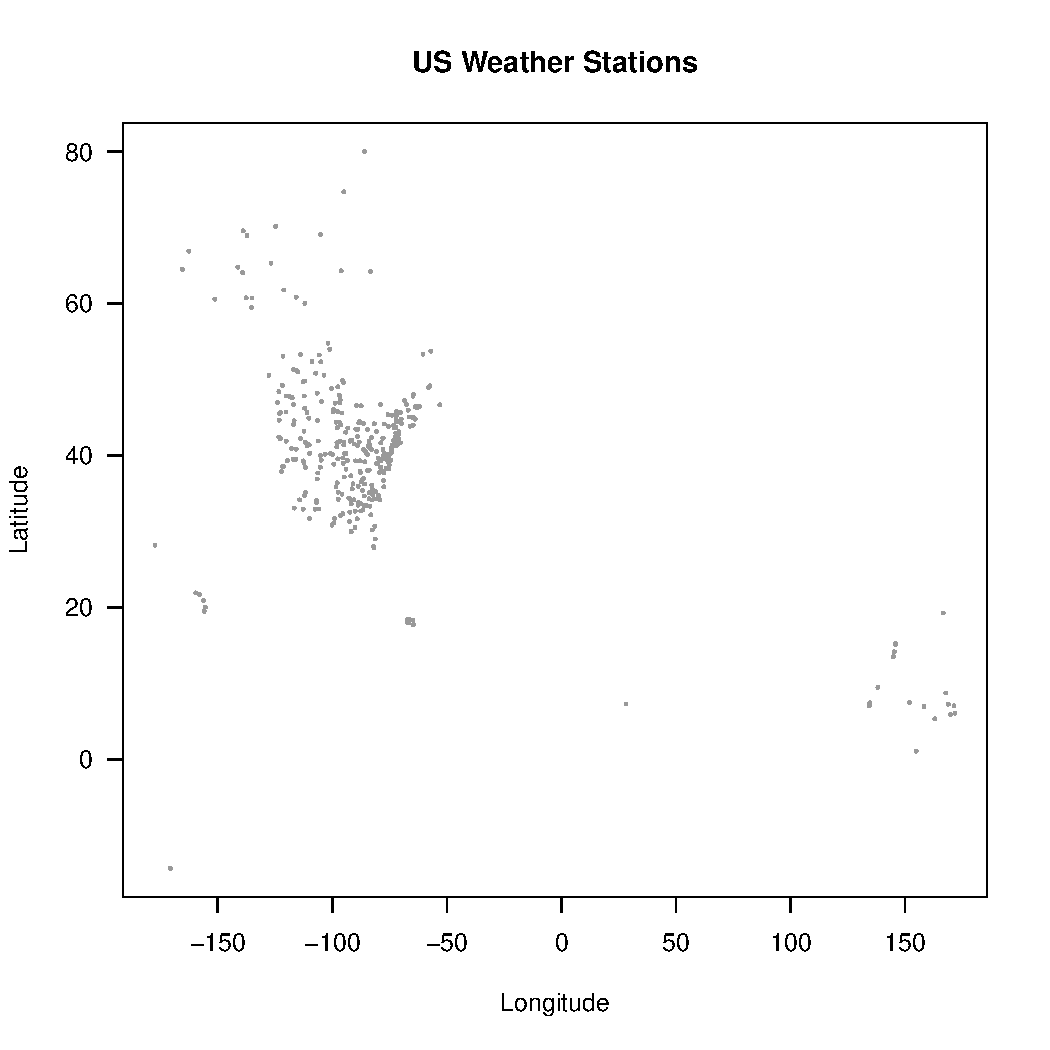
\includegraphics[width=\maxwidth]{figure/unnamed-chunk-2-1} 
\end{knitrout}


\subsection{Visualizing of Active Weather Stations with Maximum Daily Temperature Readings}

\begin{knitrout}
\definecolor{shadecolor}{rgb}{0.969, 0.969, 0.969}\color{fgcolor}\begin{kframe}
\begin{alltt}
\hlcom{# Subset data for TMAX  (Max Temperature) Element}
\hlstd{inventory.TMAX} \hlkwb{=} \hlkwd{subset}\hlstd{(inventory,} \hlkwc{subset}\hlstd{=ELEMENT}\hlopt{==}\hlstr{"TMAX"}\hlstd{)}

\hlkwd{str}\hlstd{(inventory.TMAX)}
\end{alltt}
\begin{verbatim}
## 'data.frame':	40395 obs. of  6 variables:
##  $ ID       : chr  "ACW00011604" "ACW00011647" "AE000041196" "AEM00041194" ...
##  $ LATITUDE : num  17.1 17.1 25.3 25.3 24.4 ...
##  $ LONGITUDE: num  -61.8 -61.8 55.5 55.4 54.7 ...
##  $ ELEMENT  : chr  "TMAX" "TMAX" "TMAX" "TMAX" ...
##  $ FIRSTYEAR: int  1949 1961 1944 1983 1983 1994 1973 1973 1966 1973 ...
##  $ LASTYEAR : int  1949 1961 2024 2024 2024 2024 1992 2020 2021 2020 ...
\end{verbatim}
\begin{alltt}
\hlcom{#plot(inventory.TMAX$LONGITUDE, inventory.TMAX$LATITUDE)}

\hlcom{#plot(inventory.TMAX$LONGITUDE, inventory.TMAX$LATITUDE, pch=20, cex=.4)}

\hlcom{# Selective ~Active Stations}

\hlstd{inventory.TMAX} \hlkwb{=} \hlkwd{subset}\hlstd{(inventory.TMAX,} \hlkwc{subset}\hlstd{=LASTYEAR}\hlopt{>=}\hlnum{2022}\hlstd{);} \hlkwd{str}\hlstd{(inventory.TMAX)}
\end{alltt}
\begin{verbatim}
## 'data.frame':	12745 obs. of  6 variables:
##  $ ID       : chr  "AE000041196" "AEM00041194" "AEM00041217" "AEM00041218" ...
##  $ LATITUDE : num  25.3 25.3 24.4 24.3 36.7 ...
##  $ LONGITUDE: num  55.52 55.36 54.65 55.61 3.25 ...
##  $ ELEMENT  : chr  "TMAX" "TMAX" "TMAX" "TMAX" ...
##  $ FIRSTYEAR: int  1944 1983 1983 1994 1940 1940 1958 1886 1878 1880 ...
##  $ LASTYEAR : int  2024 2024 2024 2024 2024 2024 2024 2023 2024 2024 ...
\end{verbatim}
\begin{alltt}
\hlcom{#plot(inventory.TMAX$LONGITUDE, inventory.TMAX$LATITUDE, pch=20, cex=.4, xlab="Long", ylab="Lat", las=1)}

\hlcom{#par(mfrow=c(2,2))}
\end{alltt}
\end{kframe}
\end{knitrout}

\begin{figure}
  \caption{A plot of the global weather stations. Note the increase in stations over time and spatial distribution. Austrailia has most of it's stations with 1750 start dates, but I suspect most of these stations have lots of missing data. }
  \label{fig:global-weather-stations}
\begin{knitrout}
\definecolor{shadecolor}{rgb}{0.969, 0.969, 0.969}\color{fgcolor}
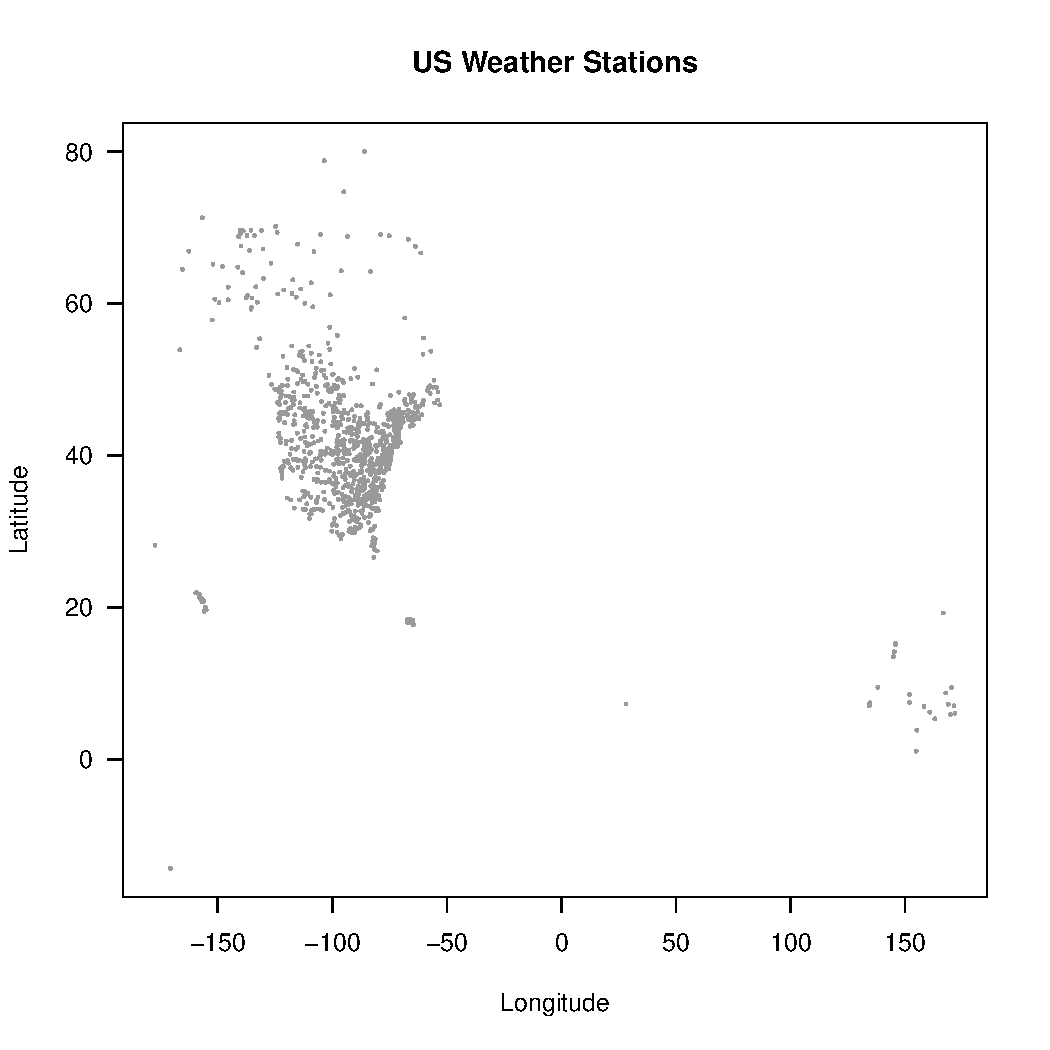
\includegraphics[width=\maxwidth]{figure/unnamed-chunk-4-1} 
\end{knitrout}
\end{figure}

\section{Creating Up-to-Date Weather Datasets}

To prepare for the project, we need to accomplish two things: 

\begin{enumerate}
  \item Select a region, i.e. State, of interest
  \item Read in the most recent EPA information on the state.
\end{enumerate}

\section{Updated Station Selection Dataset}

\subsection{Download Recent}

\subsection{States in GHCND-station Dataset}

The inventory has a list of stations and map coordinates (latitude and longitude). However, it's not easy to select a region, like a state, from the inventory. Thus, we need to merge the inventory with a dataset that includes state names.

It's a bit strange, but the dataset includes US states and Canadian Provinces, plus various territories of the US. 

\begin{knitrout}
\definecolor{shadecolor}{rgb}{0.969, 0.969, 0.969}\color{fgcolor}\begin{kframe}
\begin{alltt}
\hlstd{station_names} \hlkwb{=} \hlkwd{c}\hlstd{(}\hlstr{"ID"}\hlstd{,}             \hlcom{#  1-11   Character   11}
                  \hlstr{"LATITUDE"}\hlstd{,}       \hlcom{# 13-20   Real        8}
                  \hlstr{"LONGITUDE"}\hlstd{,}      \hlcom{# 22-30   Real        9}
                  \hlstr{"ELEVATION"}\hlstd{,}      \hlcom{# 32-37   Real        6}
                  \hlstr{"STATE"}\hlstd{,}          \hlcom{# 39-40   Character   2}
                  \hlstr{"NAME"}\hlstd{,}           \hlcom{# 42-71   Character}
                  \hlstr{"GSN FLAG"}\hlstd{,}       \hlcom{# 73-75   Character}
                  \hlstr{"HCN/CRN FLAG"}\hlstd{,}   \hlcom{# 77-79   Character}
                  \hlstr{"WMO ID"}          \hlcom{# 81-85   Character}
                   \hlstd{)}

\hlstd{Stations} \hlkwb{=} \hlkwd{read.fwf}\hlstd{(}\hlstr{"https://www.ncei.noaa.gov/pub/data/ghcn/daily/ghcnd-stations.txt"}\hlstd{,} \hlkwc{col.names}\hlstd{=station_names,} \hlkwc{fill}\hlstd{=}\hlnum{2}\hlstd{,}
        \hlkwc{widths}\hlstd{=}\hlkwd{c}\hlstd{(}\hlnum{11}\hlstd{,} \hlopt{-}\hlnum{1}\hlstd{,} \hlnum{8}\hlstd{,} \hlopt{-}\hlnum{1}\hlstd{,} \hlnum{9}\hlstd{,} \hlopt{-}\hlnum{1}\hlstd{,} \hlnum{6}\hlstd{,} \hlopt{-}\hlnum{1}\hlstd{,} \hlnum{2}\hlstd{,} \hlopt{-}\hlnum{1}\hlstd{,} \hlnum{30}\hlstd{,} \hlopt{-}\hlnum{1}\hlstd{,} \hlnum{3}\hlstd{,} \hlopt{-}\hlnum{1}\hlstd{,} \hlnum{3}\hlstd{,} \hlopt{-}\hlnum{1}\hlstd{,} \hlnum{5} \hlstd{))}

\hlcom{# NOTE: Got to be a better way to get these data!}

\hlkwd{str}\hlstd{(Stations)} \hlcom{# Missing State Name}
\end{alltt}
\begin{verbatim}
## 'data.frame':	125988 obs. of  9 variables:
##  $ ID          : chr  "ACW00011604" "ACW00011647" "AE000041196" "AEM00041194" ...
##  $ LATITUDE    : num  17.1 17.1 25.3 25.3 24.4 ...
##  $ LONGITUDE   : num  -61.8 -61.8 55.5 55.4 54.7 ...
##  $ ELEVATION   : num  10.1 19.2 34 10.4 26.8 ...
##  $ STATE       : chr  "  " "  " "  " "  " ...
##  $ NAME        : chr  "ST JOHNS COOLIDGE FLD         " "ST JOHNS                      " "SHARJAH INTER. AIRP           " "DUBAI INTL                    " ...
##  $ GSN.FLAG    : chr  "   " "   " "GSN" "   " ...
##  $ HCN.CRN.FLAG: chr  "   " "   " "   " "   " ...
##  $ WMO.ID      : int  NA NA 41196 41194 41217 41218 40930 40938 40948 40990 ...
\end{verbatim}
\begin{alltt}
\hlcom{# Read ghcnd-states.txt}

\hlstd{State_names} \hlkwb{=} \hlkwd{c}\hlstd{(}\hlstr{"STATE"}\hlstd{,} \hlcom{#         1-2    Character 2}
                \hlstr{"STATE_NAME"}\hlstd{)} \hlcom{#         4-50    Character 46}


\hlstd{States} \hlkwb{=} \hlkwd{read.fwf}\hlstd{(}\hlstr{"https://www.ncei.noaa.gov/pub/data/ghcn/daily/ghcnd-states.txt"}\hlstd{,} \hlkwc{col.names}\hlstd{=State_names,} \hlkwc{fill}\hlstd{=}\hlnum{2}\hlstd{,} \hlkwc{widths}\hlstd{=}\hlkwd{c}\hlstd{(}\hlnum{2}\hlstd{,} \hlopt{-}\hlnum{1}\hlstd{,} \hlnum{46}\hlstd{))}


\hlkwd{str}\hlstd{(States)}
\end{alltt}
\begin{verbatim}
## 'data.frame':	74 obs. of  2 variables:
##  $ STATE     : chr  "AB" "AK" "AL" "AR" ...
##  $ STATE_NAME: chr  "ALBERTA" "ALASKA" "ALABAMA                                       " "ARKANSAS" ...
\end{verbatim}
\begin{alltt}
\hlstd{StateIDs} \hlkwb{=} \hlkwd{subset}\hlstd{(Stations,} \hlkwc{select}\hlstd{=}\hlkwd{c}\hlstd{(}\hlstr{"ID"}\hlstd{,} \hlstr{"STATE"}\hlstd{))}
\hlstd{StateIDs} \hlkwb{=} \hlkwd{merge}\hlstd{(StateIDs, States,} \hlkwc{by}\hlstd{=}\hlstr{"STATE"}\hlstd{)} \hlcom{# Add State Names}

\hlstd{temp.TMAX} \hlkwb{=} \hlkwd{merge}\hlstd{(inventory.TMAX, StateIDs,} \hlkwc{by}\hlstd{=}\hlstr{"ID"}\hlstd{)}
\hlcom{# Note: Some outer join would be better, to be completed later.}

\hlstd{stations.USCan} \hlkwb{=} \hlkwd{subset}\hlstd{(temp.TMAX,} \hlkwc{subset}\hlstd{=(STATE}\hlopt{!=}\hlstr{"  "}\hlstd{))} \hlcom{# Remove Stations that STATE = blank!}
\end{alltt}
\end{kframe}
\end{knitrout}

\subsection{Select Active Stations}

How many stations are in the state? 'r nrow(stations.USCan)'!
\begin{knitrout}
\definecolor{shadecolor}{rgb}{0.969, 0.969, 0.969}\color{fgcolor}\begin{kframe}
\begin{alltt}
\hlstd{stations.active} \hlkwb{=} \hlkwd{subset}\hlstd{(stations.USCan,} \hlkwc{subset}\hlstd{=LASTYEAR}\hlopt{>=}\hlnum{2022}\hlstd{)}
\hlkwd{str}\hlstd{(stations.active)}
\end{alltt}
\begin{verbatim}
## 'data.frame':	7751 obs. of  8 variables:
##  $ ID        : chr  "AQW00061705" "CA001011500" "CA001012055" "CA001012475" ...
##  $ LATITUDE  : num  -14.3 48.9 48.8 48.4 48.4 ...
##  $ LONGITUDE : num  -171 -124 -124 -123 -123 ...
##  $ ELEMENT   : chr  "TMAX" "TMAX" "TMAX" "TMAX" ...
##  $ FIRSTYEAR : int  1966 1979 1960 1997 1991 1991 2007 1972 1970 1996 ...
##  $ LASTYEAR  : int  2024 2024 2023 2024 2024 2024 2024 2024 2022 2024 ...
##  $ STATE     : chr  "AS" "BC" "BC" "BC" ...
##  $ STATE_NAME: chr  "AMERICAN SAMOA" "BRITISH COLUMBIA" "BRITISH COLUMBIA" "BRITISH COLUMBIA" ...
\end{verbatim}
\begin{alltt}
\hlkwd{nrow}\hlstd{(stations.active)}
\end{alltt}
\begin{verbatim}
## [1] 7751
\end{verbatim}
\end{kframe}
\end{knitrout}

\subsection{Select 5 Stations for Each State}

To accomplish this, I need to do a loop to select the first 5 stations for each state.

\begin{knitrout}
\definecolor{shadecolor}{rgb}{0.969, 0.969, 0.969}\color{fgcolor}\begin{kframe}
\begin{alltt}
\hlcom{# Loop to select 5 stations for each state}
\hlcom{#stations.active.oldest = subset(stations.active, subset=FIRSTYEAR==min(FIRSTYEAR))}

\hlkwa{for}\hlstd{(i} \hlkwa{in} \hlnum{1}\hlopt{:}\hlkwd{nrow}\hlstd{(States)) \{}
  \hlstd{state.df} \hlkwb{=} \hlkwd{subset}\hlstd{(stations.active,} \hlkwc{subset}\hlstd{=STATE}\hlopt{==}\hlstd{States}\hlopt{$}\hlstd{STATE[i])}
  \hlkwa{if}\hlstd{(}\hlkwd{nrow}\hlstd{(state.df)} \hlopt{>} \hlnum{5}\hlstd{) \{}
    \hlstd{state.df} \hlkwb{=} \hlstd{state.df[}\hlkwd{order}\hlstd{(state.df}\hlopt{$}\hlstd{FIRSTYEAR),][}\hlnum{1}\hlopt{:}\hlnum{5}\hlstd{,]}
  \hlstd{\}}
  \hlkwa{if}\hlstd{(i}\hlopt{==}\hlnum{1}\hlstd{) \{}
    \hlstd{stations.active.oldest} \hlkwb{=} \hlstd{state.df}
  \hlstd{\}} \hlkwa{else} \hlstd{\{}
    \hlstd{stations.active.oldest} \hlkwb{=} \hlkwd{rbind}\hlstd{(stations.active.oldest, state.df)}
  \hlstd{\}}
\hlstd{\}}
\end{alltt}
\end{kframe}
\end{knitrout}

\section{Plot Results}

\begin{knitrout}
\definecolor{shadecolor}{rgb}{0.969, 0.969, 0.969}\color{fgcolor}\begin{kframe}
\begin{alltt}
\hlkwd{plot}\hlstd{(stations.active.oldest}\hlopt{$}\hlstd{LONGITUDE, stations.active.oldest}\hlopt{$}\hlstd{LATITUDE,} \hlkwc{pch}\hlstd{=}\hlnum{20}\hlstd{,} \hlkwc{cex}\hlstd{=}\hlnum{.4}\hlstd{,} \hlkwc{xlab}\hlstd{=}\hlstr{"Long"}\hlstd{,} \hlkwc{ylab}\hlstd{=}\hlstr{"Lat"}\hlstd{,} \hlkwc{las}\hlstd{=}\hlnum{1}\hlstd{)}
\end{alltt}
\end{kframe}
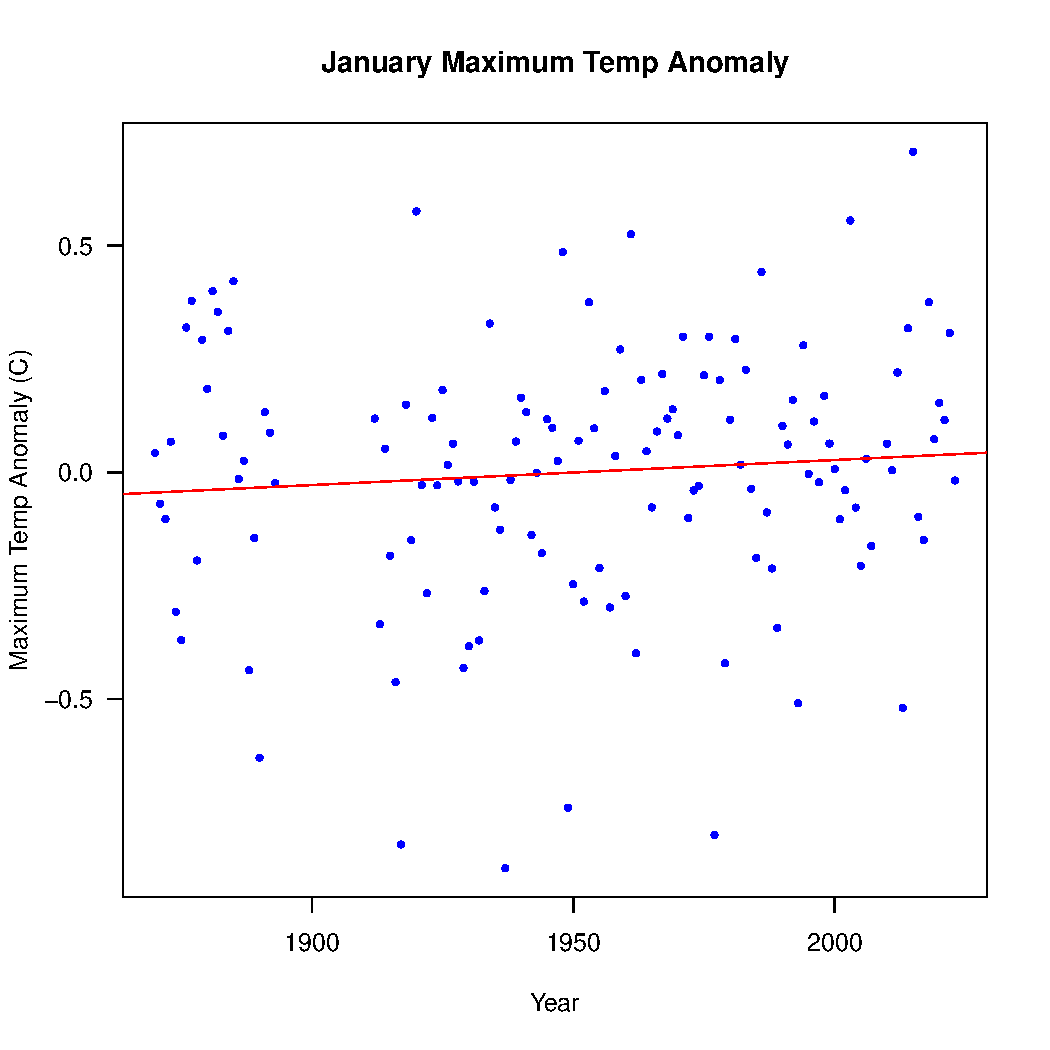
\includegraphics[width=\maxwidth]{figure/unnamed-chunk-8-1} 
\end{knitrout}

\subsection{Next Steps}


\begin{knitrout}
\definecolor{shadecolor}{rgb}{0.969, 0.969, 0.969}\color{fgcolor}\begin{kframe}
\begin{alltt}
\hlcom{# export file to csv}
\hlkwd{write.csv}\hlstd{(stations.active.oldest,} \hlkwd{here}\hlstd{(}\hlstr{"04_Regional_Climate_Trends"}\hlstd{,} \hlstr{"stations.active.oldest.csv"}\hlstd{))}
\end{alltt}
\end{kframe}
\end{knitrout}







\end{document}
